\subsection{Schallwellen} (auch noch ein Beispiel)
Schallwellen: in Gasen:
\begin{itemize}
	\item Druck- und Dichtewellen
	\item Longitudinalwellen
\end{itemize}
In Gasen und idealen Flüssigkeiten $ \nexists $ Scherkräfte, d.h. keine Kräfte $ \perp $ Bewegungsrichtung!\\
"Momentanaufnahme" einer Druckwelle:
\begin{center}
	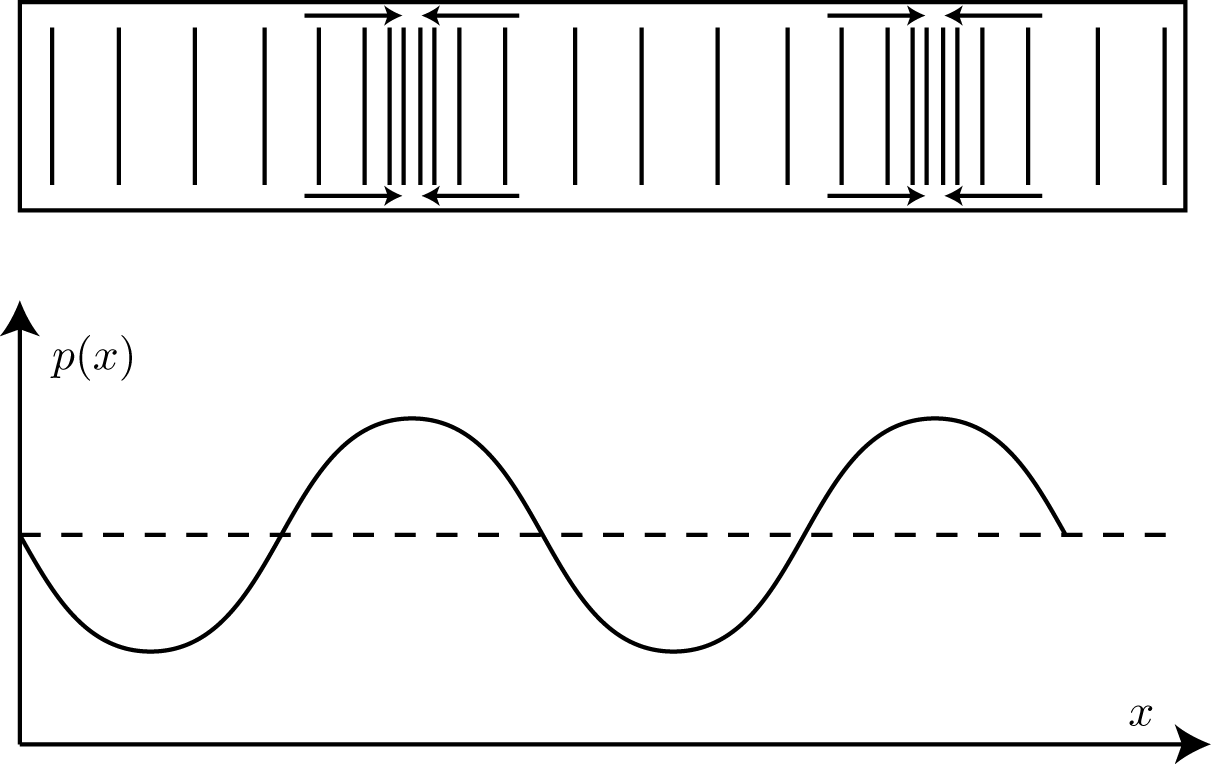
\includegraphics[width=0.7\linewidth]{skizzen/19/19B23}
\end{center}
Schwingungsknoten $ \hat{=} $ Druckband\\
Erinnerung: "Flammrohr", letzte L vor X-Mas 2015\\
Beispiel für stehende Schallwelle: Schwingungen der Luftsäule (z.B. Orgelpfeifen)
\begin{center}
	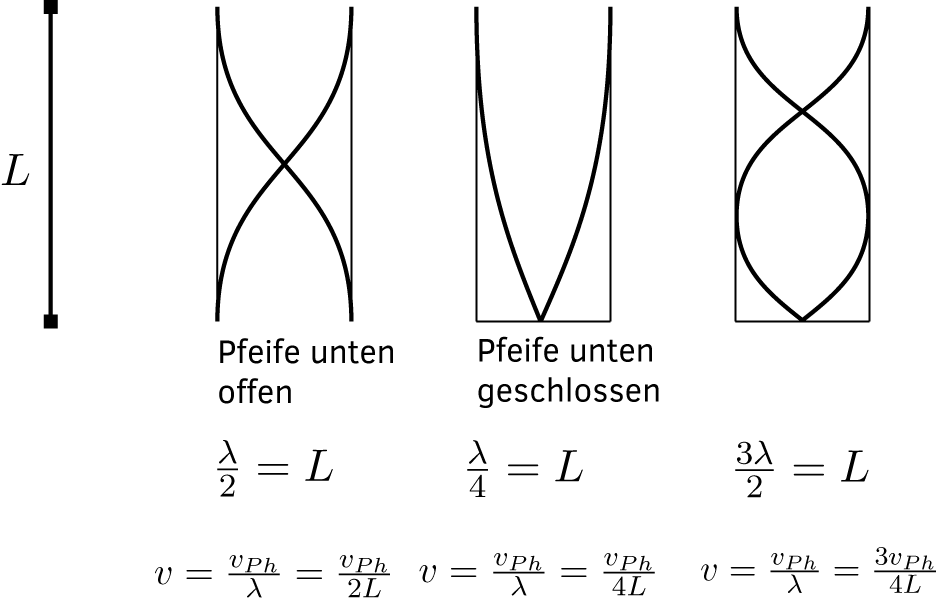
\includegraphics[width=0.7\linewidth]{skizzen/19/19B24}
\end{center}
Was bestimmt $ v_{Ph} $ von Schallwellen?\\
$ \Rightarrow $ Rücktreibende Kraft bei Druckschwankungen?\\
Seilwelle: $ \frac{\pi}{\rho} \Rightarrow \frac{d\overset{\text{Druck}}{p}}{d\rho}=v^2_{Ph}$\\
Bei adiabatischer Druckänderung  (kein Wärmeausgleich, schnell) folgt:\\
$$ \frac{dp}{d\rho} = \kappa \cdot \frac{K_B \cdot T}{m} \Rightarrow \boxed{v_{Ph} = \sqrt{\kappa\cdot\frac{K_BT}{m}}}$$\\
$ \Rightarrow $ Schallwellen sind dispersionsfrei (zum Glück)
$$ \omega = \v_{Ph} \cdot \kappa = \sqrt{\kappa\cdot\frac{K_BT}{m}} \cdot K $$
$ v_{Ph} = v_{Ph}(\kappa,T,m) $\\
Erinnerung: $ \kappa = 1 + \frac{2}{f} $ \hspace{5mm} $ f $: $ \# $ Freiheitsgrade des Moleküls\\
\enter
$ v_{Ph} $ @ 273K:\\
\begin{align*}
\text{Luft: } &N_2 \hspace{3mm}; m=28u; 2\text{-atomig}; f=5; \kappa = \frac{7}{5} \Rightarrow v_{Ph}=\SI{331}{\meter\per\second}\\
&H_2 \hspace{3mm}; m=2u; 2\text{-atomig}; f=5; \kappa = \frac{7}{5} \Rightarrow v_{Ph}=\SI{1240}{\meter\per\second} \\
\text{Helium: } &He \hspace{3mm}; m=4u; 1\text{-atomig}; f=3; \kappa = \frac{5}{3} \Rightarrow v_{Ph}=\SI{1007}{\meter\per\second}\\
&\omega= v_{Ph} \cdot K \Rightarrow \nu = \frac{v_{Ph}}{\lambda}
\end{align*}
Bei gleicher Geometrie (z.B. eines Resonators) ändert sich $ \nu $ bei Austausch des Gases: (Luft $ \rightarrow $ He : $ \nu \rightarrow \approx 3 \cdot \nu$)\\
\subsubsection{Experiment: Helium-stimme}\enter
Beachte: $ \nu = \frac{v_{Ph}(\sqrt{T})}{\lambda} $ : Temperatureinfluss auf "Stimmung" von Instrumenten \\
Vergleiche: $ \v_{Ph} $ und thermische Geschwindigkeit $ v_{th} $\\
\begin{align*}
&v_{Ph} = \sqrt{\kappa\frac{K_BT}{m}} &&; \sqrt{<v_{th}^2>} = \sqrt{3\frac{K}{m}}\\
\Rightarrow &\frac{v_{th}}{v_{Ph}}=\sqrt{\frac{3}{\kappa}} &&\Rightarrow v_{th} \approx 1,3 \cdot v_{Ph} ... 1,4 \cdot v_{Ph}\\
 v_{th}&  \text{ ist \underline{nicht }}  >>  v_{Ph} &&\Rightarrow \text{ kein schneller thermischer Ausgleich}\\
 & &&\Rightarrow \text{ Adiabatische Näherung ok!}
\end{align*}
\begin{center}
	\rule{5cm}{.2pt}
\end{center}
\subsubsection{Longitudinal Schallwellen in Festkörpern}\hfill\\
Wellengleichung: $ v_{Ph}^2 \cdot \frac{\partial^2\Psi}{\partial x^2} = \frac{\partial^2\Psi}{\partial t^2} $\\
Seilwelle: $ v_{Ph} = \sqrt{\frac{\tau}{\rho}} $\\
\subsubsection{Experiment: Schallwelle in Metallstab}
\enter
\begin{center}
	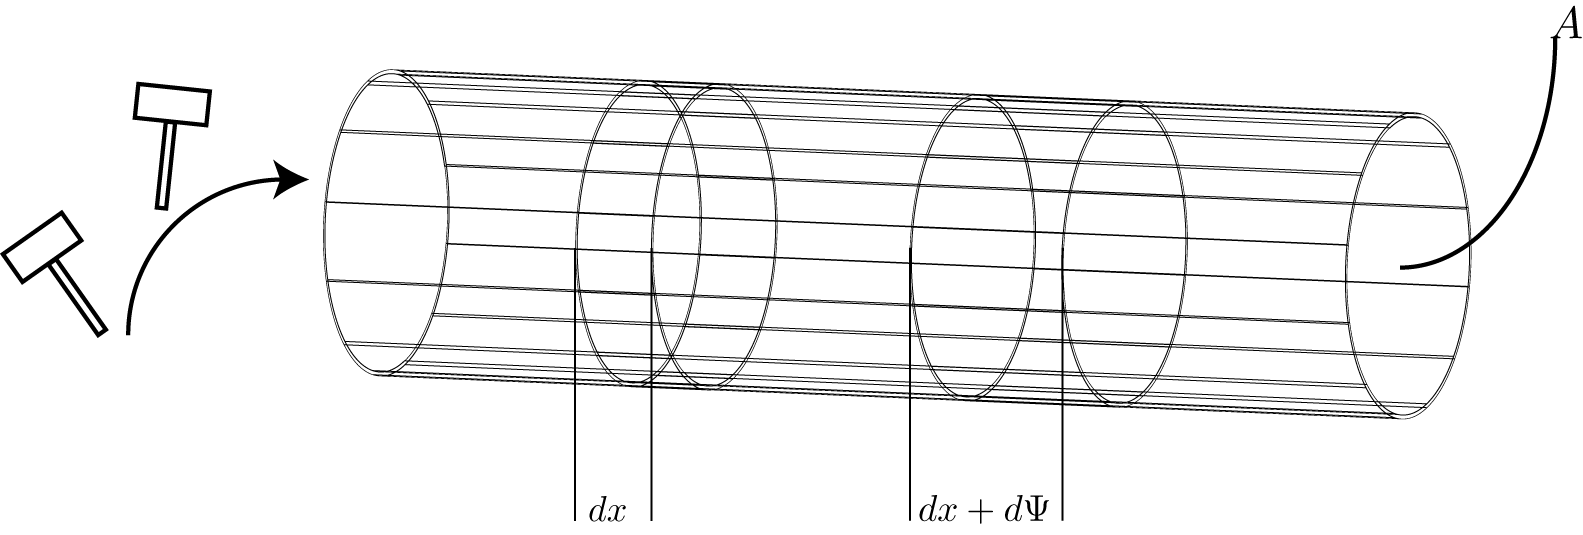
\includegraphics[width=0.7\linewidth]{skizzen/19/19B25}
\end{center}
Verformung von $ dx $ auf $ dx+x\Psi $\\
Dehnung: $ \epsilon = \frac{d\Psi}{dx} $\\
Verallgemeinerung Hook'sches Gesetz: $ \sigma = \frac{F}{A} = \underbracket{E}_{\mathclap{\text{Elasititätsmodul}}} \cdot \epsilon$\\
\begin{align*}
\rightarrow dF &= A \cdot E \cdot \frac{d\Psi}{dx}\\
\frac{dF}{dx} &= \underline{A \cdot E \cdot \frac{d^2\Psi}{dx^2}} \hspace{2cm} \text{(*)}
\end{align*}
\begin{align*}
\text{Beschleunigung auf Massenelement: }  dm = \rho\cdot dV = \rho\cdot A \cdot dx \\
dF = dm \cdot \frac{\partial^2\Psi}{\partial t^2} = \rho \cdot A \cdot dx \cdot \frac{\partial^2\Psi}{\partial t^2}\\
\frac{dF}{dx} = \rho \cdot A \cdot \frac{\partial^2\Psi}{\partial t^2} \hspace{2cm} \text{(**)}
\enter
\end{align*}
$$ \text{(*) (**) : } \boxed{\frac{E}{\rho} \cdot \frac{\partial^2\Psi}{\partial x^2} =  \frac{\partial^2 \Psi}{\partial t^2}} $$
\begin{center}
	Wellengleichung mit $ \underline{\underline{v_{Phi} = \sqrt{\frac{E}{\rho}}}} $ ; dispersionsfrei
\end{center}
$$ \underline{\underline{\omega = \sqrt{\frac{E}{\rho}} \cdot K}} $$
\begin{align*}
\text{Typische Werte (Stahl): } &E \approx \SI{2E11}{\newton\per\meter^2} \hspace{2cm} (200\si{\giga\pascal}) \\
&\rho = \SI{8E3}{\kilogram\per\meter^3}\\
\Rightarrow v_{Ph} = \sqrt{\frac{E}{\rho}} \approx \SI{5E3}{\meter\per\second} >> v_{Ph} \text{ (Luft)}
\end{align*}

In Festkörpern sind wegen Schwerkraft auch transversal Wellen Möglich: \hspace{2cm} $ G $ : Schermodul

$$ \underline{\underline{\Rightarrow v_{Ph} = \sqrt{\frac{G}{\rho}}}} $$

\subsubsection{Wasserwellen}
\enter
($ \Rightarrow $ Entstehung: Handout)
\kommentar{Handout muss hier noch nachgetragen werden.}
\begin{center}
	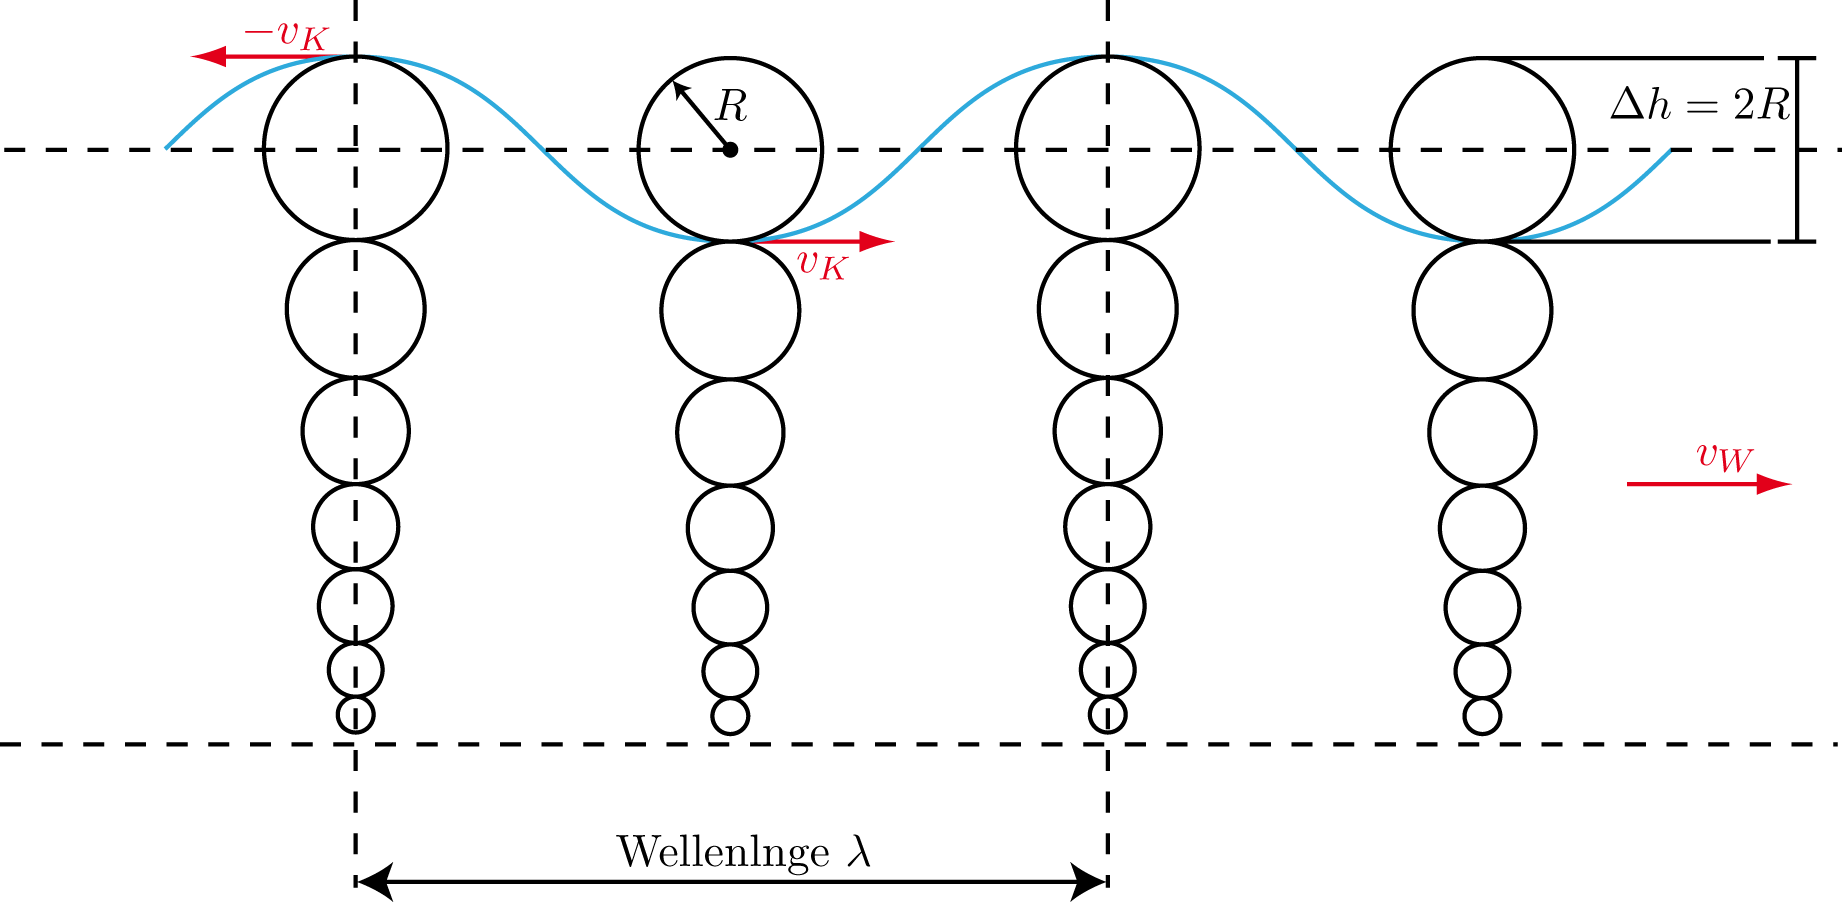
\includegraphics[width=0.7\linewidth]{skizzen/19/19B26}
\end{center}
Geschwindigkeit auf Wellenberg: $ v_{Berg} = v_W - v_K$\\
Geschwindigkeit im Wellental: $ v_{Tal} = v_{W} + v_{K} $\\
\begin{tcolorbox}[width=\textwidth*3/5,colback={White}]
Im Mittel kein Materialtransport
\end{tcolorbox}
Zunahme an kinetischer Energie vom Berg zum Tal:
$$ \Delta E^{kin} = E_{Tal}^{kin} - E_{Berg}^{kin} = \frac{1}{2} \cdot m (v_{Tal}^2 - v_{Berg}^2) 2 \cdot m \cdot v_{W} \cdot v_{K}$$
($ m $ : Masse der Wellenfront)\\
"Verlust" an potenzieller Energie:
$$ \Delta E ^{pot} = 2mgR $$
\begin{align*}
\Delta E^{pot}  = \Delta E ^{kin} \Leftarrow\\
\Rightarrow v_W = \sqrt{\frac{g\cdot\lambda_W}{2\pi}}
\end{align*}
\kommentar{"zu Hause zeigen", muss noch gemacht werden}
Schwere-wellen zeigen ausgeprägte Dispersion:
\begin{align*}
\lambda_w = \SI{10}{\meter} &\Rightarrow v_W = \SI{4}{\meter\per\second}\\
\lambda_w = \SI{1000}{\meter} &\Rightarrow v_W = \SI{40}{\meter\per\second}
\end{align*}
Für kleinere $ \lambda $ : Oberflächenspannung $ \sigma $ berücksichtigen\\
zusätzlich: Einfluss endlicher Wassertiefe berücksichtigen
\begin{center}
	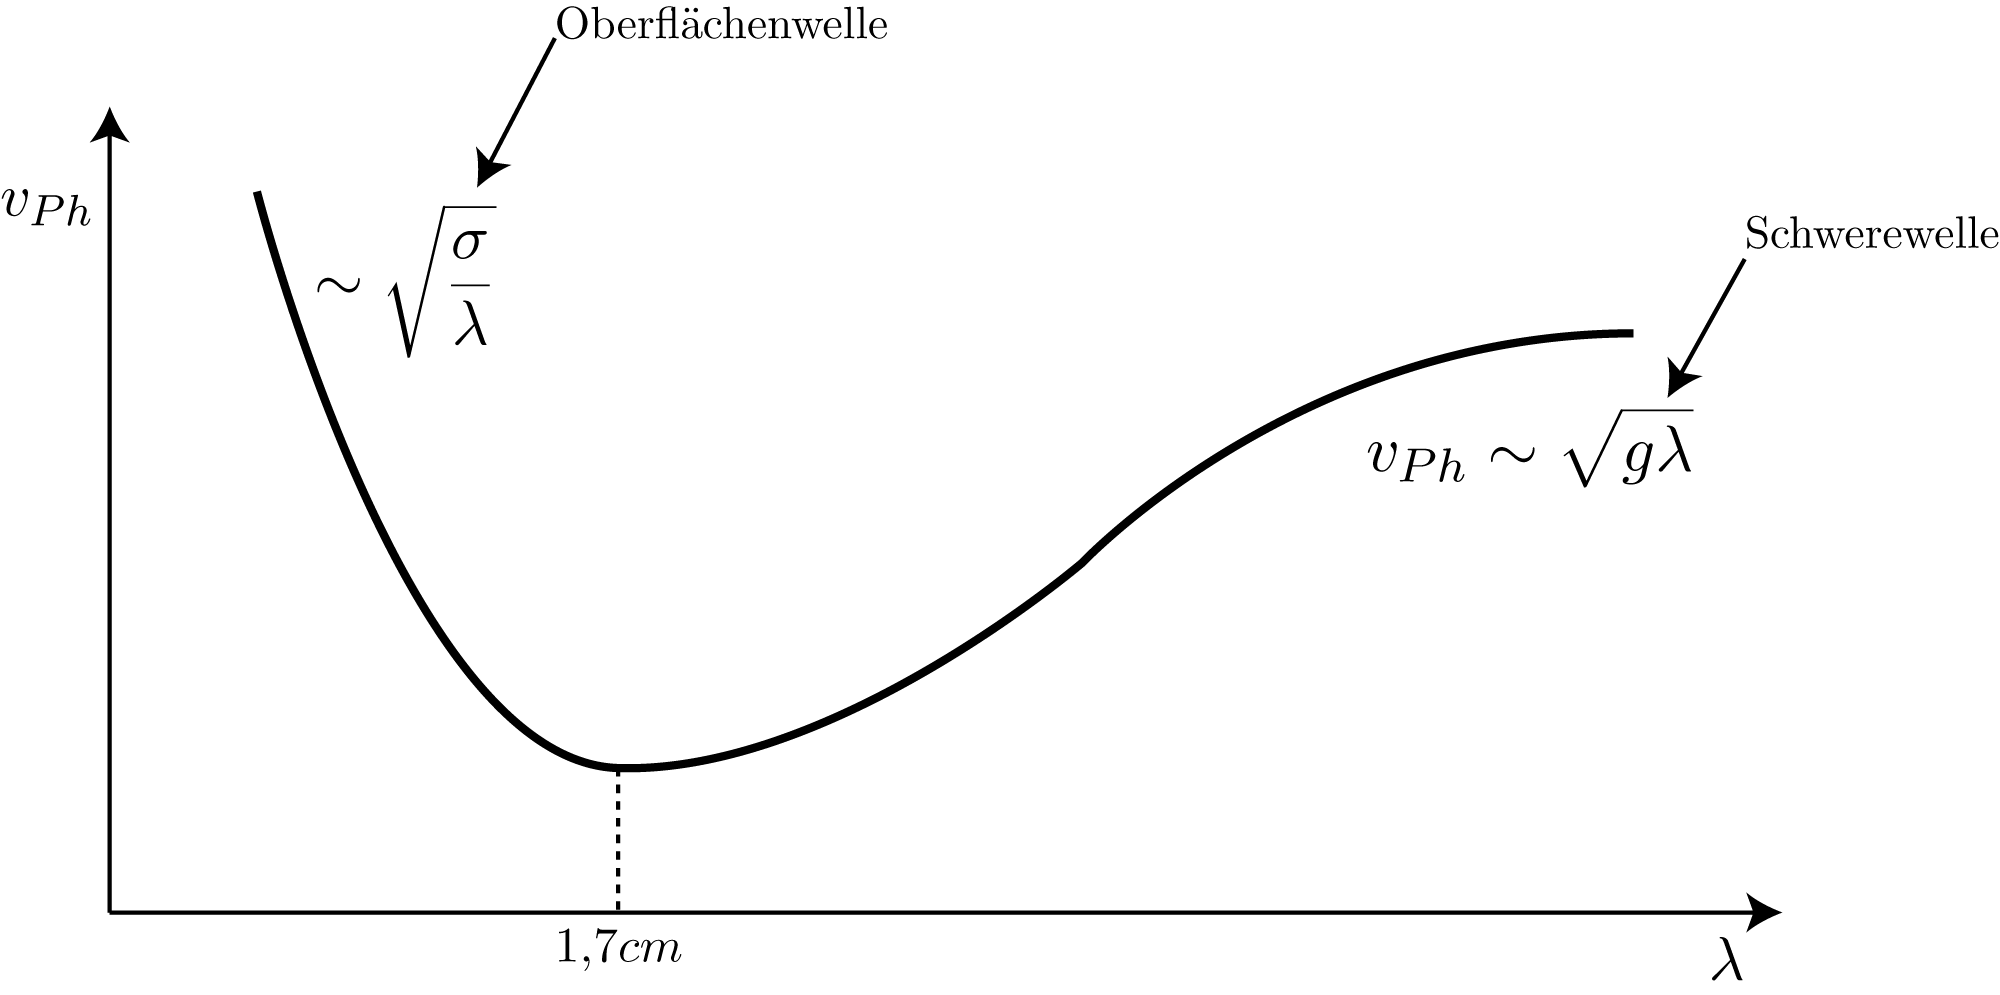
\includegraphics[width=0.7\linewidth]{skizzen/19/19B27}
\end{center}
Es gilt allgemein (Komplexe Rechnung).\\
$$ v_{Ph} = \sqrt{\frac{g\cdot\lambda_W}{2\pi}+\frac{2\pi\sigma}{\underbrace{\rho\cdot\lambda_W}_{\text{Oberfläche}}}} \cdot \overset{(A)^{1/2}}{\underset{h: \text{ Wassertiefe}}{\sqrt{\frac{1-\exp(-2\cdot K \cdot h)}{1+\exp(-2 \cdot K \cdot h)}}}}$$

\paragraph{Seichtwasserwellen:}
ab $  n \leq \frac{\lambda_W}{4} $ muss endliche Tiefe berücksichtigt werden!\\
$$\text{(A): } \frac{1-\exp(-2Kh)}{1+\exp(-2Kh)} \overset{n<<\frac{2\pi}{K}}{\longrightarrow} \frac{1-(1-2Kh)}{1+(1-2Kh)} = \frac{2Kh}{2-2Kh} \approx Kh$$
Beschränkung auf Nicht-Oberflächenwelle:\\
$$ \rightarrow v_{Ph} = \sqrt{\frac{g\cdot\lambda_W}{2\pi}} \sqrt{\frac{2\pi}{\lambda_W}\cdot h} = \sqrt{g \cdot h} $$
Keine Dispersion für Flachwasserwelle; \underline{$ v_{Ph}  $ hängt nur von $ h $ ab!!}\\
$ \Rightarrow $ Das ist der Grund für Entstehung von Brandung und Tsünamos!\\
Experiment: Tiefwasser $ \rightarrow $ Flachwasserwelle\\
\begin{center}
	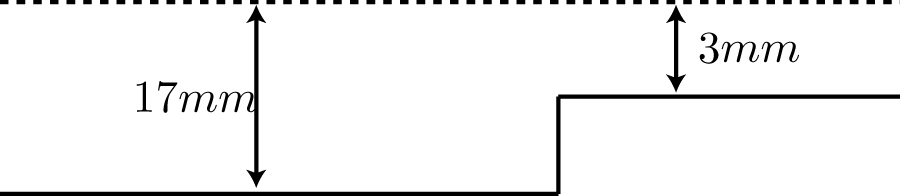
\includegraphics[width=0.5\linewidth]{skizzen/19/19B28}
\end{center}
$$ v_{Ph}  = \sqrt{g\cdot h}; \lambda_1 = \frac{v_{Ph}}{\nu} = \frac{\SI{0,41}{\meter\per\second}}{\nu}; \lambda_2 = \frac{\SI{0,17}{\meter\per\second}}{\nu} $$
$ \nu  = const.$ (Erregerfrequenz)
Entstehung von Tsünamos:\\
$ \lambda=\SI{100}{\kilo\meter} - \SI{500}{\kilo\meter} $ (z.B. durch Seebeben)\\
$ \Rightarrow $ Tsünamos sind überall Flachwasserwellen (Wellenhöhe: $ <\SI{1}{\meter} $)\\
$ v_{Ph} = \sqrt{g\cdot h} $ in Ozeanen ($ h \approx \SI{5000}{\meter} $) : $ \vDash_{Ph} =\SI{780}{\kilo\meter\per\hour} $\\
Periodendauer: $ T=\SI{7,5}{\minute} ... \SI{38}{\minute} $\\
In flachem Wasser ($ h=\SI{5}{-meter} $) reduziert sich $ v_{Ph}  $ auf ca $ 1/30 $
$$ v_{Ph}  \approx \SI{26}{\kilo\meter\per\hour}$$
$ \lambda $ reduziert sich ebenfalls auf $ 1/30 $
\begin{tcolorbox} [colback = {White}, outer arc=0mm, sharp corners]
	Da $ E_{km} $ erhalten bleibt, nimmt die Amplitude drastisch zu!!
\end{tcolorbox}
